\documentclass[11pt]{article}
\usepackage{mathblatt}
% gesetzt von werkzeuge/setzer.py (Sorte selbst) aus dem Lernweg A5D
% und den Bankzeilen; Muster bau/proben/2026-10-09/hypotenuse-muster.
\usepackage{enumitem}
\usepackage{adjustbox,varwidth}
\newgeometry{a4paper,margin=18mm,top=15mm,bottom=20mm,footskip=9mm}
\pagestyle{fancy}\fancyhf{}\renewcommand{\headrulewidth}{0pt}
\fancyfoot[L]{\footnotesize\color{mbgrau}A5D \textperiodcentered{} Brüche: kürzen und erweitern}
\fancyfoot[R]{\footnotesize\color{mbgrau}\thepage}
\setlength{\parskip}{3pt}
\renewcommand{\kreuz}[1]{\mbox{$\square$\ #1}\quad}
\newcommand{\kreuzl}[1]{\par\hangindent1.4em\hangafter1\noindent$\square$\ #1}
\newcommand{\aufg}[3]{\par\noindent\makebox[0pt][r]{#3}\begin{minipage}[t]{\linewidth}#1\end{minipage}\par}
\newcommand{\aufgg}[4]{\par\noindent\makebox[0pt][r]{#4}\begin{minipage}[t]{0.6\linewidth}\vspace{0pt}#1\end{minipage}\hfill
  \begin{minipage}[t]{0.37\linewidth}\vspace{0pt}\centering #2\end{minipage}\par}
\newcommand{\nr}[1]{\makebox[7mm][l]{\textbf{#1}}}
\newcommand{\lsg}[3]{\par\noindent\begin{minipage}[t]{9mm}\textbf{#1}\end{minipage}%
  \begin{minipage}[t]{52mm}\raggedright\bfseries\boldmath #2\end{minipage}\hspace{3mm}%
  \begin{minipage}[t]{\dimexpr\linewidth-64mm\relax}\raggedright\small #3\end{minipage}\par\vspace{4pt}}
\newlength{\kr}
\makeatletter
\newcommand{\karomerk}[2]{\protected@write\@auxout{}{\string\karoseite{#1}{#2}{\thepage}}}
\newcommand{\karoseite}[3]{\expandafter\xdef\csname karo@#1@#2\endcsname{#3}}
\newcommand{\karohinweis}[3]{\karomerk{h}{#1}\ifcsname karo@k@#1\endcsname
  \ifnum\csname karo@k@#1\endcsname=0\csname karo@h@#1\endcsname\relax#2\else#3\fi
  \else#3\fi}
\makeatother
\begin{document}

\noindent{\LARGE\bfseries Brüche: kürzen und erweitern}\par\smallskip
\noindent{\small\color{mbgrau}Selbstlernheft Klasse 6 \textperiodcentered{} mit Lösungsheft \textperiodcentered{} Kennung A5D}\par\medskip
\noindent\textbf{So nutzt du das Heft:} Lies im Abschnitt das Beispiel. Rechne dann die Aufgaben der Reihe nach und vergleiche jede sofort mit dem Lösungsheft. Kreuze „kann ich“ an, wenn du die letzte Aufgabe (\emph{Ziel}) allein schaffst.\par
\noindent Mehr Aufgaben zu einem Abschnitt: Kennung deinem Nachhilfelehrer schicken (z.\,B. „A5D mehr B“).\par\medskip
{\arrayrulecolor{mbgrau}\renewcommand{\arraystretch}{1.3}
\noindent\begin{tabular}{|>{\bfseries}p{10mm}|p{112mm}|>{\raggedleft\arraybackslash}p{10mm}|>{\centering\arraybackslash}p{14mm}|}\hline
\rowcolor{black!8} & \textbf{Abschnitt} & \textbf{Seite} & \textbf{kann ich}\\\hline
A & Erweitern und kürzen & \pageref{s:A} & $\square$\\\hline
B & Vollständig kürzen & \pageref{s:B} & $\square$\\\hline
C & Auf einen gemeinsamen Nenner bringen & \pageref{s:C} & $\square$\\\hline
D & Brüche größer als 1: gemischte Zahlen & \pageref{s:D} & $\square$\\\hline
T & Probetest & \pageref{s:T} & $\square$\\\hline
\end{tabular}}\par\bigskip

\begin{tcolorbox}[colback=mbkasten,colframe=mbgrau,boxrule=0.5pt,arc=1mm,left=3mm,right=3mm,top=2mm,bottom=2mm,title={\bfseries Formel auf einen Blick},coltitle=black,colbacktitle=black!10]
{\Large $\dfrac{Z}{N} = \dfrac{Z \cdot k}{N \cdot k}$ \qquad $\dfrac{Z}{N} = \dfrac{Z : k}{N : k}$ \qquad $\dfrac{Z}{N} = Z : N$}\par\medskip
In Worten: Zähler und Nenner mit derselben Zahl malnehmen (erweitern) oder durch dieselbe Zahl teilen (kürzen): Der Bruch bleibt gleich groß.\par\medskip
\end{tcolorbox}
\medskip\noindent\textbf{Typische Fehler – so nicht}\par\smallskip
\noindent\nr{$\times$}Nur den Zähler erweitert: $\dfrac{3}{8}$ mit 2 ist $\dfrac{6}{16}$, nicht $\dfrac{6}{8}$.\par
\noindent\nr{$\times$}Mit einer Zahl gekürzt, die nur oben oder nur unten teilt: $\dfrac{9}{20}$ lässt sich nicht durch 3 kürzen, denn 20 steht nicht in der Dreierreihe.\par
\clearpage\label{s:A}\noindent\colorbox{black!12}{\makebox[10mm]{\Large\bfseries\strut A}}\hspace{3mm}{\Large\bfseries Erweitern und kürzen}\par\smallskip
\noindent Teilst du jedes Teil eines Streifens in gleich viele Stücke, werden Zähler und Nenner mit derselben Zahl malgenommen – die graue Fläche bleibt gleich groß. Das heißt \textbf{erweitern}; rückwärts gelesen heißt es \textbf{kürzen}.\par\medskip
\noindent\textbf{Formel}\par\nopagebreak\noindent\hspace*{4mm}\begin{minipage}{\dimexpr\linewidth-4mm\relax}erweitern: $\dfrac{Z}{N} = \dfrac{Z \cdot k}{N \cdot k}$ \qquad kürzen: $\dfrac{Z}{N} = \dfrac{Z : k}{N : k}$ \qquad $k$ = neuer Nenner $:$ alter Nenner\end{minipage}\par\medskip
\noindent\textbf{Beispiel}\quad Beide Streifen sind gleich lang. Der obere zeigt $\frac{3}{4}$. Der untere ist in 8 gleiche Teile geteilt. Wie viele Teile musst du unten färben, damit gleich viel grau ist?\par\smallskip
\noindent\begin{minipage}[t]{0.6\linewidth}\vspace{0pt}\par\noindent\hangindent6mm\hangafter1\makebox[6mm][l]{\textbf{1}}Jedes Viertel ist unten in 2 Teile geteilt: Aus 4 Teilen werden $4 \cdot 2 = 8$.\par\smallskip\par\noindent\hangindent6mm\hangafter1\makebox[6mm][l]{\textbf{2}}Aus 3 grauen Teilen werden $3 \cdot 2 = 6$. Färbe 6 Teile.\par\smallskip\par\noindent\hangindent6mm\hangafter1\makebox[6mm][l]{\textbf{3}}$\dfrac{3}{4} = \dfrac{3 \cdot 2}{4 \cdot 2} = \dfrac{6}{8}$. Das heißt: mit 2 \textbf{erweitert}.\par\smallskip\par\noindent\hangindent6mm\hangafter1\makebox[6mm][l]{\textbf{4}}Von unten nach oben gelesen: $\dfrac{6}{8} = \dfrac{6 : 2}{8 : 2} = \dfrac{3}{4}$. Das heißt: mit 2 \textbf{gekürzt}.\par\smallskip\end{minipage}\hfill
\begin{minipage}[t]{0.37\linewidth}\vspace{0pt}\centering 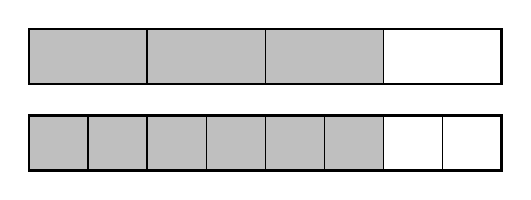
\begin{tikzpicture}[line cap=round]\fill[black!25] (0.000,0.00) rectangle (0.750,0.70);\fill[black!25] (0.750,0.00) rectangle (1.500,0.70);\draw[line width=0.4pt] (0.750,0.00) -- (0.750,0.70);\fill[black!25] (1.500,0.00) rectangle (2.250,0.70);\draw[line width=0.4pt] (1.500,0.00) -- (1.500,0.70);\fill[black!25] (2.250,0.00) rectangle (3.000,0.70);\draw[line width=0.4pt] (2.250,0.00) -- (2.250,0.70);\fill[black!25] (3.000,0.00) rectangle (3.750,0.70);\draw[line width=0.4pt] (3.000,0.00) -- (3.000,0.70);\fill[black!25] (3.750,0.00) rectangle (4.500,0.70);\draw[line width=0.4pt] (3.750,0.00) -- (3.750,0.70);\draw[line width=0.4pt] (4.500,0.00) -- (4.500,0.70);\draw[line width=0.4pt] (5.250,0.00) -- (5.250,0.70);\draw[line width=0.9pt] (0,0.00) rectangle (6.0,0.70);\fill[black!25] (0.000,1.10) rectangle (1.500,1.80);\fill[black!25] (1.500,1.10) rectangle (3.000,1.80);\draw[line width=0.4pt] (1.500,1.10) -- (1.500,1.80);\fill[black!25] (3.000,1.10) rectangle (4.500,1.80);\draw[line width=0.4pt] (3.000,1.10) -- (3.000,1.80);\draw[line width=0.4pt] (4.500,1.10) -- (4.500,1.80);\draw[line width=0.9pt] (0,1.10) rectangle (6.0,1.80);\end{tikzpicture}\end{minipage}\par\medskip
\noindent\textbf{Aufgaben}\hspace{1em}{\small\color{mbgrau}\karohinweis{A}{Rechne unten im Karo.}{Rechne auf einem extra Blatt.} Vergleiche jede Aufgabe gleich mit dem Lösungsheft.}\par\smallskip
\aufgg{\hangindent7mm\hangafter1\nr{1.}Beide Streifen sind gleich lang. Der obere zeigt $\frac{2}{5}$. Färbe im unteren Streifen gleich viel. Welcher Bruch steht dann unten?}{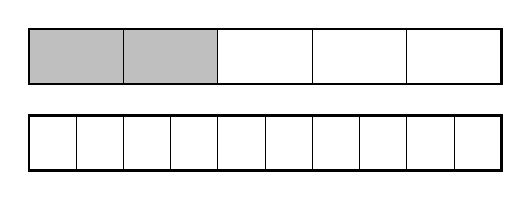
\begin{tikzpicture}[line cap=round]\draw[line width=0.4pt] (0.600,0.00) -- (0.600,0.70);\draw[line width=0.4pt] (1.200,0.00) -- (1.200,0.70);\draw[line width=0.4pt] (1.800,0.00) -- (1.800,0.70);\draw[line width=0.4pt] (2.400,0.00) -- (2.400,0.70);\draw[line width=0.4pt] (3.000,0.00) -- (3.000,0.70);\draw[line width=0.4pt] (3.600,0.00) -- (3.600,0.70);\draw[line width=0.4pt] (4.200,0.00) -- (4.200,0.70);\draw[line width=0.4pt] (4.800,0.00) -- (4.800,0.70);\draw[line width=0.4pt] (5.400,0.00) -- (5.400,0.70);\draw[line width=0.9pt] (0,0.00) rectangle (6.0,0.70);\fill[black!25] (0.000,1.10) rectangle (1.200,1.80);\fill[black!25] (1.200,1.10) rectangle (2.400,1.80);\draw[line width=0.4pt] (1.200,1.10) -- (1.200,1.80);\draw[line width=0.4pt] (2.400,1.10) -- (2.400,1.80);\draw[line width=0.4pt] (3.600,1.10) -- (3.600,1.80);\draw[line width=0.4pt] (4.800,1.10) -- (4.800,1.80);\draw[line width=0.9pt] (0,1.10) rectangle (6.0,1.80);\end{tikzpicture}}{}{}
\medskip
\aufg{\hangindent7mm\hangafter1\nr{2.}Erweitert oder gekürzt – und mit welcher Zahl? \par\vspace{3pt} a)~$\dfrac{4}{9} = \dfrac{20}{45}$ \qquad b)~$\dfrac{21}{28} = \dfrac{3}{4}$ \qquad c)~$\dfrac{5}{8} = \dfrac{40}{64}$}{}{}
\medskip
\aufg{\hangindent7mm\hangafter1\nr{3.}Erweitere mit der Zahl in Klammern. \par\vspace{3pt} a)~$\dfrac{3}{5}$ (mit 4) \qquad b)~$\dfrac{5}{6}$ (mit 3) \qquad c)~$\dfrac{7}{9}$ (mit 10)}{}{}
\medskip
\aufg{\hangindent7mm\hangafter1\nr{4.}Kürze mit der Zahl in Klammern. \par\vspace{3pt} a)~$\dfrac{20}{24}$ (mit 4) \qquad b)~$\dfrac{15}{35}$ (mit 5) \qquad c)~$\dfrac{24}{42}$ (mit 6)}{}{}
\medskip
\aufg{\hangindent7mm\hangafter1\nr{5.}Lena bricht ihren Schokoriegel in 4 gleiche Stücke und isst 3 davon. Tom bricht einen gleich großen Riegel in 12 gleiche Stücke und isst 9 davon. Wer hat mehr gegessen?}{}{{\scriptsize\color{mbgrau}Ziel\hspace{2mm}}}
\medskip
\par\vspace{3mm}\setlength{\kr}{\dimexpr\pagegoal-\pagetotal-10mm\relax}%
\ifdim\kr>12mm\karomerk{k}{A}\noindent{\scriptsize\color{mbgrau}Platz zum Rechnen}\par\nointerlineskip\vspace{1mm}\noindent
\begin{tikzpicture}\clip (0,0) rectangle ({\linewidth-0.5mm},\kr);\draw[black!16,line width=0.3pt,step=5mm] (0,0) grid (\linewidth,\kr);\end{tikzpicture}\fi\par
\clearpage\label{s:B}\noindent\colorbox{black!12}{\makebox[10mm]{\Large\bfseries\strut B}}\hspace{3mm}{\Large\bfseries Vollständig kürzen}\par\smallskip
\noindent Vollständig gekürzt ist ein Bruch, wenn keine Zahl außer 1 Zähler und Nenner zugleich teilt. Kürze in kleinen Schritten oder gleich mit der größten Zahl, die beide teilt.\par\medskip
\noindent\textbf{Formel}\par\nopagebreak\noindent\hspace*{4mm}\begin{minipage}{\dimexpr\linewidth-4mm\relax}Teilt 2, 3, 5 oder 7 Zähler und Nenner? Dann kürzen. \par {\small Bruchteil einer Größe: erst beides in dieselbe Einheit, z.\,B. 1\,h $= 60$\,min.}\end{minipage}\par\medskip
\noindent\textbf{Beispiel}\quad Kürze $\frac{30}{42}$ vollständig.\par\smallskip
\noindent\par\noindent\hangindent6mm\hangafter1\makebox[6mm][l]{\textbf{1}}Beide Zahlen sind gerade: durch 2. \ $\dfrac{30}{42} = \dfrac{15}{21}$\par\smallskip\par\noindent\hangindent6mm\hangafter1\makebox[6mm][l]{\textbf{2}}15 und 21 stehen beide in der Dreierreihe: durch 3. \ $\dfrac{15}{21} = \dfrac{5}{7}$\par\smallskip\par\noindent\hangindent6mm\hangafter1\makebox[6mm][l]{\textbf{3}}5 und 7 teilt keine Zahl außer 1. Fertig: $\dfrac{30}{42} = \dfrac{5}{7}$\par\smallskip\par\noindent\hangindent6mm\hangafter1\makebox[6mm][l]{\textbf{4}}Schneller geht es mit einem Schritt: durch 6, die größte Zahl, die 30 und 42 teilt.\par\smallskip\par\medskip
\noindent\textbf{Aufgaben}\hspace{1em}{\small\color{mbgrau}\karohinweis{B}{Rechne unten im Karo.}{Rechne auf einem extra Blatt.} Vergleiche jede Aufgabe gleich mit dem Lösungsheft.}\par\smallskip
\aufg{\hangindent7mm\hangafter1\nr{1.}Kürze vollständig. \par\vspace{3pt} a)~$\dfrac{6}{8}$ \qquad b)~$\dfrac{10}{15}$ \qquad c)~$\dfrac{8}{20}$}{}{}
\medskip
\aufg{\hangindent7mm\hangafter1\nr{2.}Kürze vollständig. Prüfe nach jedem Kürzen, ob es noch weiter geht. \par\vspace{3pt} a)~$\dfrac{18}{24}$ \qquad b)~$\dfrac{36}{60}$ \qquad c)~$\dfrac{48}{72}$ \par\vspace{3pt} d)~Kürze in einem Schritt: Welche größte Zahl teilt 36 und 48? Kürze $\dfrac{36}{48}$ mit ihr.}{}{}
\medskip
\aufgg{\hangindent7mm\hangafter1\nr{3.}Die Figur besteht aus gleich großen Kästchen. Welcher Anteil der Figur ist grau? Gib ihn vollständig gekürzt an.}{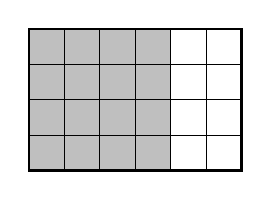
\begin{tikzpicture}[line cap=round]\fill[black!25] (0.00,1.35) rectangle (0.45,1.80);\fill[black!25] (0.45,1.35) rectangle (0.90,1.80);\fill[black!25] (0.90,1.35) rectangle (1.35,1.80);\fill[black!25] (1.35,1.35) rectangle (1.80,1.80);\fill[black!25] (0.00,0.90) rectangle (0.45,1.35);\fill[black!25] (0.45,0.90) rectangle (0.90,1.35);\fill[black!25] (0.90,0.90) rectangle (1.35,1.35);\fill[black!25] (1.35,0.90) rectangle (1.80,1.35);\fill[black!25] (0.00,0.45) rectangle (0.45,0.90);\fill[black!25] (0.45,0.45) rectangle (0.90,0.90);\fill[black!25] (0.90,0.45) rectangle (1.35,0.90);\fill[black!25] (1.35,0.45) rectangle (1.80,0.90);\fill[black!25] (0.00,0.00) rectangle (0.45,0.45);\fill[black!25] (0.45,0.00) rectangle (0.90,0.45);\fill[black!25] (0.90,0.00) rectangle (1.35,0.45);\fill[black!25] (1.35,0.00) rectangle (1.80,0.45);\draw[line width=0.4pt] (0,0) grid[step=0.45] (2.70,1.80);\draw[line width=0.9pt] (0,0) rectangle (2.70,1.80);\end{tikzpicture}}{}{}
\medskip
\aufg{\hangindent7mm\hangafter1\nr{4.}Welcher Bruchteil des Ganzen ist das? Gib ihn vollständig gekürzt an. \par a)~50 min von 1 h \qquad b)~750 g von 1 kg \qquad c)~35 cm von 1 m}{}{}
\medskip
\aufg{\hangindent7mm\hangafter1\nr{5.}Tim hat im Test 21 von 28 Punkten. Er sagt: „Das sind drei Viertel der Punkte.“ Hat er recht?}{}{{\scriptsize\color{mbgrau}Ziel\hspace{2mm}}}
\medskip
\par\vspace{3mm}\setlength{\kr}{\dimexpr\pagegoal-\pagetotal-10mm\relax}%
\ifdim\kr>12mm\karomerk{k}{B}\noindent{\scriptsize\color{mbgrau}Platz zum Rechnen}\par\nointerlineskip\vspace{1mm}\noindent
\begin{tikzpicture}\clip (0,0) rectangle ({\linewidth-0.5mm},\kr);\draw[black!16,line width=0.3pt,step=5mm] (0,0) grid (\linewidth,\kr);\end{tikzpicture}\fi\par
\clearpage\label{s:C}\noindent\colorbox{black!12}{\makebox[10mm]{\Large\bfseries\strut C}}\hspace{3mm}{\Large\bfseries Auf einen gemeinsamen Nenner bringen}\par\smallskip
\noindent Für einen bestimmten Nenner rechnest du zuerst aus, mit welcher Zahl du erweitern musst. Zwei Brüche macht man \textbf{gleichnamig}, indem man beide auf denselben Nenner erweitert.\par\medskip
\noindent\textbf{Formel}\par\nopagebreak\noindent\hspace*{4mm}\begin{minipage}{\dimexpr\linewidth-4mm\relax}gemeinsamer Nenner: eine Zahl, die in beiden Einmaleins-Reihen steht \par {\small Es geht immer: Nenner mal Nenner.} \par\smallskip Nenner 100 heißt Prozent: $\dfrac{3}{10} = \dfrac{30}{100} = 30\,\%$.\end{minipage}\par\medskip
\noindent\textbf{Beispiel}\quad Mache $\frac{3}{4}$ und $\frac{5}{6}$ gleichnamig.\par\smallskip
\noindent\par\noindent\hangindent6mm\hangafter1\makebox[6mm][l]{\textbf{1}}Gemeinsamen Nenner suchen. Sechserreihe: 6, 12 – und 12 steht auch in der Viererreihe.\par\smallskip\par\noindent\hangindent6mm\hangafter1\makebox[6mm][l]{\textbf{2}}Mit welcher Zahl erweitern? \ $12 : 4 = 3$ \ und \ $12 : 6 = 2$\par\smallskip\par\noindent\hangindent6mm\hangafter1\makebox[6mm][l]{\textbf{3}}$\dfrac{3}{4} = \dfrac{3 \cdot 3}{4 \cdot 3} = \dfrac{9}{12}$ \ und \ $\dfrac{5}{6} = \dfrac{5 \cdot 2}{6 \cdot 2} = \dfrac{10}{12}$\par\smallskip\par\medskip
\noindent\textbf{Aufgaben}\hspace{1em}{\small\color{mbgrau}\karohinweis{C}{Rechne unten im Karo.}{Rechne auf einem extra Blatt.} Vergleiche jede Aufgabe gleich mit dem Lösungsheft.}\par\smallskip
\aufg{\hangindent7mm\hangafter1\nr{1.}Schreibe mit dem Nenner 24. \par\vspace{3pt} a)~$\dfrac{2}{3}$ \qquad b)~$\dfrac{5}{8}$ \qquad c)~$\dfrac{7}{12}$}{}{}
\medskip
\aufg{\hangindent7mm\hangafter1\nr{2.}Schreibe mit dem Nenner 100 und gib den Anteil in Prozent an ($\frac{1}{100} = 1\,\%$). \par\vspace{3pt} a)~$\dfrac{3}{10}$ \qquad b)~$\dfrac{7}{20}$ \qquad c)~$\dfrac{12}{25}$}{}{}
\medskip
\aufg{\hangindent7mm\hangafter1\nr{3.}Mache gleichnamig. Ein Nenner steckt schon im anderen. \par\vspace{3pt} a)~$\dfrac{2}{3}$ und $\dfrac{7}{9}$ \qquad b)~$\dfrac{1}{4}$ und $\dfrac{5}{12}$ \qquad c)~$\dfrac{3}{5}$ und $\dfrac{11}{20}$}{}{}
\medskip
\aufg{\hangindent7mm\hangafter1\nr{4.}Mache gleichnamig. \par\vspace{3pt} a)~$\dfrac{1}{6}$ und $\dfrac{3}{4}$ \qquad b)~$\dfrac{2}{5}$ und $\dfrac{1}{3}$ \qquad c)~$\dfrac{5}{8}$ und $\dfrac{7}{12}$}{}{}
\medskip
\aufg{\hangindent7mm\hangafter1\nr{5.}Jonas hat beim Training 21 von 25 Elfmetern verwandelt, Mia 17 von 20. Wer trifft besser? Vergleiche die Anteile in Prozent.}{}{{\scriptsize\color{mbgrau}Ziel\hspace{2mm}}}
\medskip
\par\vspace{3mm}\setlength{\kr}{\dimexpr\pagegoal-\pagetotal-10mm\relax}%
\ifdim\kr>12mm\karomerk{k}{C}\noindent{\scriptsize\color{mbgrau}Platz zum Rechnen}\par\nointerlineskip\vspace{1mm}\noindent
\begin{tikzpicture}\clip (0,0) rectangle ({\linewidth-0.5mm},\kr);\draw[black!16,line width=0.3pt,step=5mm] (0,0) grid (\linewidth,\kr);\end{tikzpicture}\fi\par
\clearpage\label{s:D}\noindent\colorbox{black!12}{\makebox[10mm]{\Large\bfseries\strut D}}\hspace{3mm}{\Large\bfseries Brüche größer als 1: gemischte Zahlen}\par\smallskip
\noindent Ist der Zähler größer als der Nenner, ist der Bruch mehr als ein Ganzes. Der Bruchstrich ist ein Geteilt-Zeichen: Zähler $:$ Nenner ergibt die Ganzen, der Rest bleibt als Bruch stehen.\par\medskip
\noindent\textbf{Formel}\par\nopagebreak\noindent\hspace*{4mm}\begin{minipage}{\dimexpr\linewidth-4mm\relax}$\dfrac{Z}{N} = Z : N$ \qquad zurück: $G\dfrac{z}{N} = \dfrac{G \cdot N + z}{N}$ \par\smallskip In Worten: Ganze mal Nenner plus Zähler, Nenner bleibt. \par\smallskip {\small Typischer Fehler: $2\dfrac{3}{4}$ ist weder $\dfrac{23}{4}$ noch $\dfrac{6}{4}$, sondern $\dfrac{2 \cdot 4 + 3}{4} = \dfrac{11}{4}$.}\end{minipage}\par\medskip
\noindent\textbf{Beispiel}\quad Schreibe $\frac{17}{5}$ als gemischte Zahl.\par\smallskip
\noindent\begin{minipage}[t]{0.6\linewidth}\vspace{0pt}\par\noindent\hangindent6mm\hangafter1\makebox[6mm][l]{\textbf{1}}Wie viele Ganze? \ $17 : 5 = 3$ Rest $2$\par\smallskip\par\noindent\hangindent6mm\hangafter1\makebox[6mm][l]{\textbf{2}}3 ganze Streifen und 2 Fünftel: \ $\dfrac{17}{5} = 3\dfrac{2}{5}$\par\smallskip\par\noindent\hangindent6mm\hangafter1\makebox[6mm][l]{\textbf{3}}Probe rückwärts: $3 \cdot 5 + 2 = 17$, also $3\dfrac{2}{5} = \dfrac{17}{5}$.\par\smallskip\end{minipage}\hfill
\begin{minipage}[t]{0.37\linewidth}\vspace{0pt}\centering 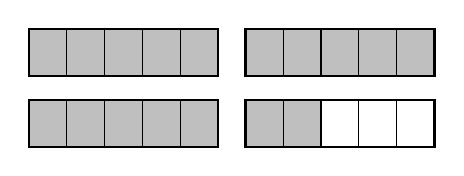
\begin{tikzpicture}[line cap=round]\fill[black!25] (0.000,0.00) rectangle (0.480,0.60);\fill[black!25] (0.480,0.00) rectangle (0.960,0.60);\draw[line width=0.4pt] (0.480,0.00) -- (0.480,0.60);\fill[black!25] (0.960,0.00) rectangle (1.440,0.60);\draw[line width=0.4pt] (0.960,0.00) -- (0.960,0.60);\fill[black!25] (1.440,0.00) rectangle (1.920,0.60);\draw[line width=0.4pt] (1.440,0.00) -- (1.440,0.60);\fill[black!25] (1.920,0.00) rectangle (2.400,0.60);\draw[line width=0.4pt] (1.920,0.00) -- (1.920,0.60);\draw[line width=0.9pt] (0.000,0.00) rectangle (2.400,0.60);\fill[black!25] (2.750,0.00) rectangle (3.230,0.60);\fill[black!25] (3.230,0.00) rectangle (3.710,0.60);\draw[line width=0.4pt] (3.230,0.00) -- (3.230,0.60);\fill[black!25] (3.710,0.00) rectangle (4.190,0.60);\draw[line width=0.4pt] (3.710,0.00) -- (3.710,0.60);\fill[black!25] (4.190,0.00) rectangle (4.670,0.60);\draw[line width=0.4pt] (4.190,0.00) -- (4.190,0.60);\fill[black!25] (4.670,0.00) rectangle (5.150,0.60);\draw[line width=0.4pt] (4.670,0.00) -- (4.670,0.60);\draw[line width=0.9pt] (2.750,0.00) rectangle (5.150,0.60);\fill[black!25] (0.000,-0.90) rectangle (0.480,-0.30);\fill[black!25] (0.480,-0.90) rectangle (0.960,-0.30);\draw[line width=0.4pt] (0.480,-0.90) -- (0.480,-0.30);\fill[black!25] (0.960,-0.90) rectangle (1.440,-0.30);\draw[line width=0.4pt] (0.960,-0.90) -- (0.960,-0.30);\fill[black!25] (1.440,-0.90) rectangle (1.920,-0.30);\draw[line width=0.4pt] (1.440,-0.90) -- (1.440,-0.30);\fill[black!25] (1.920,-0.90) rectangle (2.400,-0.30);\draw[line width=0.4pt] (1.920,-0.90) -- (1.920,-0.30);\draw[line width=0.9pt] (0.000,-0.90) rectangle (2.400,-0.30);\fill[black!25] (2.750,-0.90) rectangle (3.230,-0.30);\fill[black!25] (3.230,-0.90) rectangle (3.710,-0.30);\draw[line width=0.4pt] (3.230,-0.90) -- (3.230,-0.30);\draw[line width=0.4pt] (3.710,-0.90) -- (3.710,-0.30);\draw[line width=0.4pt] (4.190,-0.90) -- (4.190,-0.30);\draw[line width=0.4pt] (4.670,-0.90) -- (4.670,-0.30);\draw[line width=0.9pt] (2.750,-0.90) rectangle (5.150,-0.30);\end{tikzpicture}\end{minipage}\par\medskip
\noindent\textbf{Aufgaben}\hspace{1em}{\small\color{mbgrau}\karohinweis{D}{Rechne unten im Karo.}{Rechne auf einem extra Blatt.} Vergleiche jede Aufgabe gleich mit dem Lösungsheft.}\par\smallskip
\aufg{\hangindent7mm\hangafter1\nr{1.}Schreibe als gemischte Zahl. \par\vspace{3pt} a)~$\dfrac{7}{2}$ \qquad b)~$\dfrac{11}{3}$ \qquad c)~$\dfrac{23}{4}$}{}{}
\medskip
\aufg{\hangindent7mm\hangafter1\nr{2.}Schreibe als Bruch. \par\vspace{3pt} a)~$1\dfrac{3}{4}$ \qquad b)~$2\dfrac{5}{6}$ \qquad c)~$4\dfrac{2}{9}$}{}{}
\medskip
\aufg{\hangindent7mm\hangafter1\nr{3.}Schreibe als Bruch. Ist er größer als 1, schreibe ihn auch als gemischte Zahl. \par a)~$5 : 8$ \qquad b)~$9 : 4$ \qquad c)~$20 : 6$}{}{}
\medskip
\aufg{\hangindent7mm\hangafter1\nr{4.}Ein Film dauert 135 Minuten. Wie viele Stunden sind das? Schreibe als gemischte Zahl.}{}{}
\medskip
\aufg{\hangindent7mm\hangafter1\nr{5.}Für das Klassenfrühstück werden 14 Baguettes gerecht auf 4 Tische verteilt. Wie viele Baguettes bekommt jeder Tisch? Wie schneidet man die übrigen?}{}{{\scriptsize\color{mbgrau}Ziel\hspace{2mm}}}
\medskip
\par\vspace{3mm}\setlength{\kr}{\dimexpr\pagegoal-\pagetotal-10mm\relax}%
\ifdim\kr>12mm\karomerk{k}{D}\noindent{\scriptsize\color{mbgrau}Platz zum Rechnen}\par\nointerlineskip\vspace{1mm}\noindent
\begin{tikzpicture}\clip (0,0) rectangle ({\linewidth-0.5mm},\kr);\draw[black!16,line width=0.3pt,step=5mm] (0,0) grid (\linewidth,\kr);\end{tikzpicture}\fi\par
\clearpage\label{s:T}\noindent\colorbox{black!12}{\makebox[10mm]{\Large\bfseries\strut T}}\hspace{3mm}{\Large\bfseries Probetest}\par\smallskip
\noindent Gemischt, ohne Beispiel. Etwa 20 Minuten.\par\medskip
\noindent\textbf{Aufgaben}\hspace{1em}{\small\color{mbgrau}\karohinweis{T}{Rechne unten im Karo.}{Rechne auf einem extra Blatt.} Vergleiche jede Aufgabe gleich mit dem Lösungsheft.}\par\smallskip
\aufg{\hangindent7mm\hangafter1\nr{1.}Ergänze die fehlende Zahl. \par\vspace{3pt} a)~$\dfrac{3}{8} = \dfrac{\square}{40}$ \qquad b)~$\dfrac{28}{35} = \dfrac{4}{\square}$ \qquad c)~$\dfrac{5}{\square} = \dfrac{30}{42}$}{}{}
\medskip
\aufg{\hangindent7mm\hangafter1\nr{2.}Kürze vollständig. \par\vspace{3pt} a)~$\dfrac{24}{32}$ \qquad b)~$\dfrac{45}{75}$ \qquad c)~$\dfrac{36}{54}$}{}{}
\medskip
\aufg{\hangindent7mm\hangafter1\nr{3.}Mache gleichnamig. \par\vspace{3pt} a)~$\dfrac{5}{6}$ und $\dfrac{4}{9}$ \qquad b)~$\dfrac{3}{10}$ und $\dfrac{1}{4}$}{}{}
\medskip
\aufg{\hangindent7mm\hangafter1\nr{4.}Schreibe um. \par\vspace{3pt} a)~$\dfrac{29}{6}$ als gemischte Zahl \qquad b)~$3\dfrac{3}{8}$ als Bruch \qquad c)~$13 : 5$ als gemischte Zahl}{}{}
\medskip
\aufgg{\hangindent7mm\hangafter1\nr{5.}Die Figur besteht aus gleich großen Kästchen. Welcher Anteil der Fläche ist grau? Gib ihn als vollständig gekürzten Bruch und in Prozent an.}{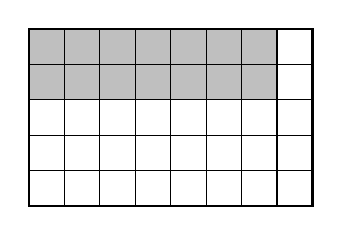
\begin{tikzpicture}[line cap=round]\fill[black!25] (0.00,1.80) rectangle (0.45,2.25);\fill[black!25] (0.45,1.80) rectangle (0.90,2.25);\fill[black!25] (0.90,1.80) rectangle (1.35,2.25);\fill[black!25] (1.35,1.80) rectangle (1.80,2.25);\fill[black!25] (1.80,1.80) rectangle (2.25,2.25);\fill[black!25] (2.25,1.80) rectangle (2.70,2.25);\fill[black!25] (2.70,1.80) rectangle (3.15,2.25);\fill[black!25] (0.00,1.35) rectangle (0.45,1.80);\fill[black!25] (0.45,1.35) rectangle (0.90,1.80);\fill[black!25] (0.90,1.35) rectangle (1.35,1.80);\fill[black!25] (1.35,1.35) rectangle (1.80,1.80);\fill[black!25] (1.80,1.35) rectangle (2.25,1.80);\fill[black!25] (2.25,1.35) rectangle (2.70,1.80);\fill[black!25] (2.70,1.35) rectangle (3.15,1.80);\draw[line width=0.4pt] (0,0) grid[step=0.45] (3.60,2.25);\draw[line width=0.9pt] (0,0) rectangle (3.60,2.25);\end{tikzpicture}}{}{}
\medskip
\aufg{\hangindent7mm\hangafter1\nr{6.}Beim Sportfest gibt es eine Urkunde, wenn man mindestens drei Viertel der möglichen Punkte holt. Ole hat 33 von 44 Punkten, Ida 26 von 36 Punkten. Wer bekommt eine Urkunde?}{}{{\scriptsize\color{mbgrau}Ziel\hspace{2mm}}}
\medskip
\par\vspace{3mm}\setlength{\kr}{\dimexpr\pagegoal-\pagetotal-10mm\relax}%
\ifdim\kr>12mm\karomerk{k}{T}\noindent{\scriptsize\color{mbgrau}Platz zum Rechnen}\par\nointerlineskip\vspace{1mm}\noindent
\begin{tikzpicture}\clip (0,0) rectangle ({\linewidth-0.5mm},\kr);\draw[black!16,line width=0.3pt,step=5mm] (0,0) grid (\linewidth,\kr);\end{tikzpicture}\fi\par
\end{document}
